\chapter{绪论}

\section{研究背景}

\begin{wrapfigure}{r}{0.5\linewidth}
    \centering
        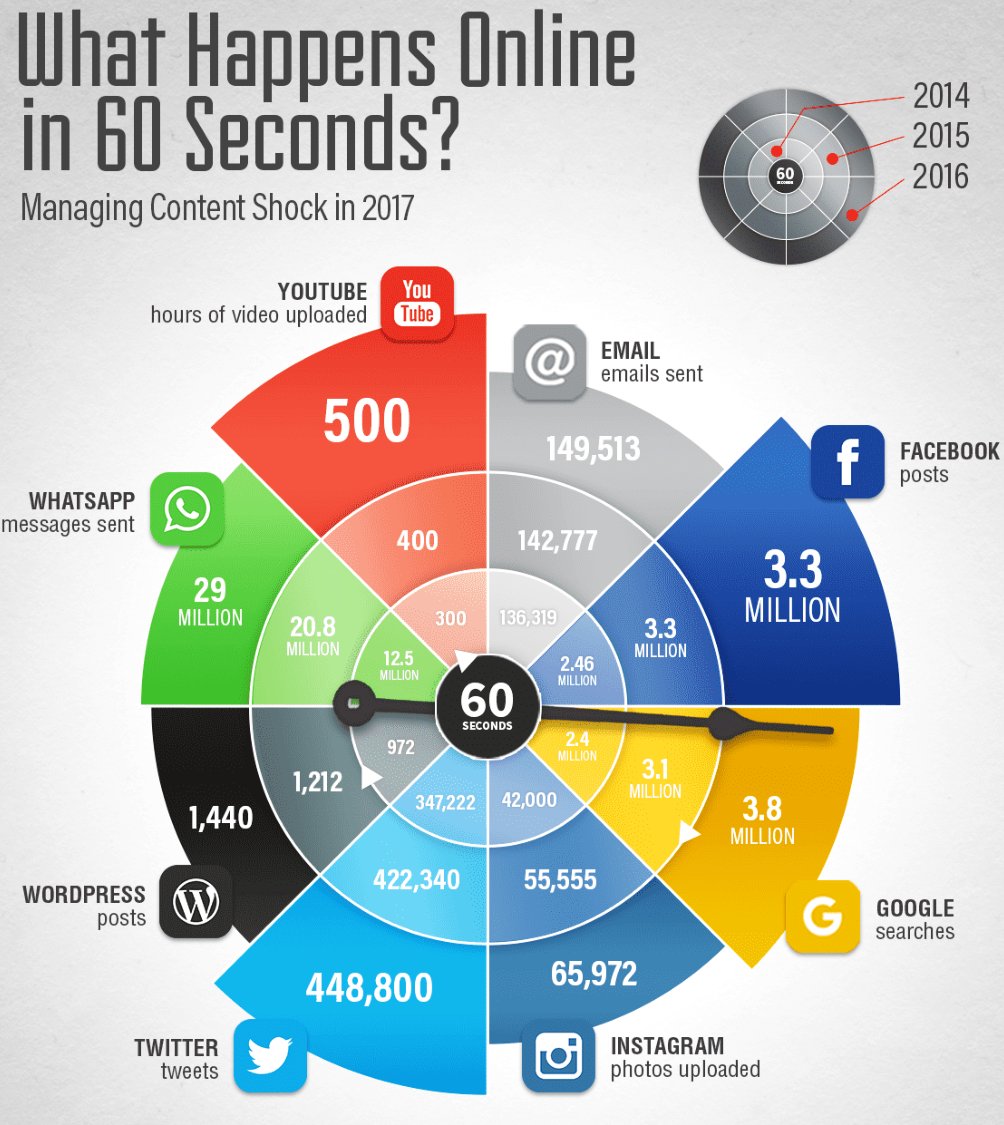
\includegraphics[width=0.95\linewidth]{chapter1/res/media_statistics.pdf}
    \captionof{figure}{大数据时代下图像视频等媒体数据呈现爆炸式增长}
    \label{ch1:fig:media_statistics}
\end{wrapfigure}

视觉是人类感知外界客观世界的主要信息来源,而计算机视觉技术旨在让机器能够像人一样感知物理世界。计算机视觉技术的发展和进步,是众多人机交互技术的基石,也是人类社会迈向真正人工智能时代至关重要的一步。目前,随着互联网技术、社交媒体技术及数字媒体设备的快速发展和普及,图像、动态图、视频等视觉媒体数据已经呈现爆炸式增长。如图~\ref{ch1:fig:media_statistics}所示\footnote{https://www.smartinsights.com/internet-marketing-statistics/happens-online-60-seconds/},截止到2016年,视频分享网站YouTube每分钟上传约500小时视频数据,图像分享社区Instagram每分钟上传约65972张图像数据。面对海量的视觉媒体数据,利用计算机视觉技术对媒体数据进行感知、理解和推理,从而实现对海量视觉媒体数据的快速检索和利用,对便利人们的日常生活、推动社会的进步有着十分重大的意义和应用价值。

另一方面,如图~\ref{ch1:fig:datasets_examples}所示,随着近年来众多大规模人工标注的图像和视频数据集的出现~\cite{lin2014microsoft,russakovsky2015imagenet,krishna2017visual,karpathy2014large,miech2019howto100m}和深度学习技术的突破~\cite{lecun2015deep,krizhevsky2012imagenet},基于深度学习的计算机视觉技术已经取得了长足的进步。例如,在大规模图像分类数据集ImageNet上,Top-1类别的分类准确率高达88.4\%、Top-5类别的分类准确率高达98.7\%~\cite{xie2019self}。然而,现有的计算机视觉技术还远远不能实现大规模的落地应用,这主要原因是由于日常生活中的媒体数据中的视觉场景通常包含大量的物体以及物体间的交互,而对复杂视觉场景的识别和理解本身存在巨大挑战。

\begin{figure}[t]
    \centering
        \includegraphics[width=0.95\linewidth]{chapter1/res/datasets_examples.pdf}
    \caption{众多大规模人工标注的图像和视频数据集推动计算机视觉的发展}
    \label{ch1:fig:datasets_examples}
\end{figure}

具体来说,对复杂视觉场景进行识别和理解,主要包含四个层次:对场景内单个物体的识别(\textbf{物体识别})、对场景内所有物体以及物体间的视觉关系的识别(\textbf{场景识别})、对整个视觉场景内容的理解(\textbf{场景理解})、以及在整个视觉场景理解的基础上进行知识推理(\textbf{场景推理})。本文将针对这四个不同层次的场景理解,逐步地对复杂视觉场景的识别、检测和推理进行研究。如图~\ref{ch1:fig:scene_understanding}所示,本文的关键技术线路主要包括物体分类、场景图生成、视觉描述生成、视觉检索和视觉问答等具体研究任务:

\begin{figure}[t]
    \centering
        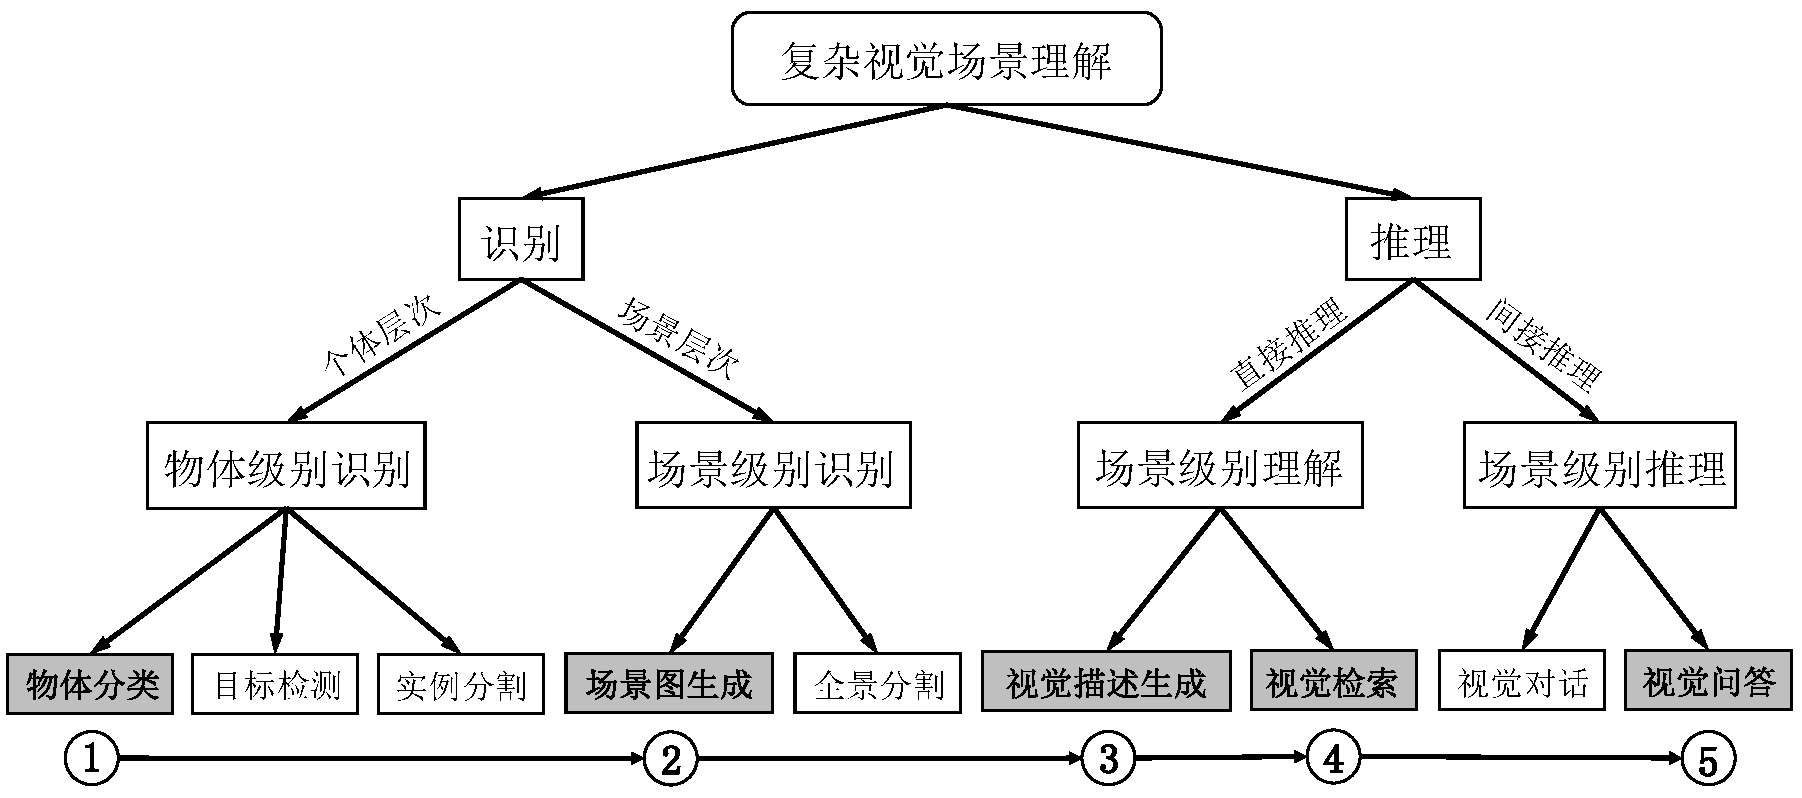
\includegraphics[width=0.95\linewidth]{chapter1/res/scene_understanding.pdf}
    \centering
    \caption{复杂场景识别、检测和推理的关键技术路线}
    \label{ch1:fig:scene_understanding}
\end{figure}

\begin{asparaenum}
\item \textbf{物体识别}:视觉场景理解的首要步骤就是对场景内包含的单个物体进行个体层次的识别。作为计算机视觉领域中一个最基本的问题,个体层次的物体识别结果将直接影响后续对整个视觉场景进行场景层次的识别、理解和推理的结果。根据物体识别的粒度,物体识别通常可以分为物体分类、目标检测、实例分割等具体任务。其中物体分类任务~\cite{russakovsky2015imagenet}的目标是对物体进行多类别分类,而目标检测任务~\cite{ren2015faster,liu2016ssd,redmon2016you}和实例分割任务~\cite{he2017mask}需要在物体分类的基础上,同时对物体的大致边框位置或精确像素位置进行定位。随着卷积神经网络(Convolutional Neural Network, CNN)的发展,在理想实验条件下(即每个类别的训练样本足够充足),物体识别技术已经可以达到较高的准确率。然而,在日常生活中,大量的类别缺乏足够的训练样本。例如,在大规模图像分类数据集ImageNet中,除了最常见的1000类图像以外,在剩余的21814个类别中,有296个类别只有一张训练样本图像~\cite{russakovsky2015imagenet}。为了让物体识别扩展到更加接近实际应用的场景中,基于少样本(Few-Shot Learning, FSL)~\cite{fei2006one}或零样本(Zero-Shot Learning, ZSL)~\cite{lampert2009learning}的物体识别逐渐成为近年来的研究热点。尤其是零样本物体分类问题中,目前的模型普遍存在属性丢失的问题(semantic loss),这大大限制模型的迁移能力。本文主要聚集在零样本物体分类中,研究如何尽可能多地保持物体属性,提升模型在不同测试类别中的迁移能力。

\item \textbf{场景识别}:对整个场景进行理解,除了需要对场景中所有的单个物体进行识别外,还需要对场景中所有物体间的视觉关系(场景图生成~\cite{johnson2015image})和所有不规则物体(全景分割~\cite{kirillov2019panoptic})进行识别。尤其对于复杂场景来说,通常包含大量的视觉关系(visual relationship),而这些视觉关系本身也可以提供丰富的语义间的内在联系,反过来帮助物体的识别。结合所有的物体以及物体间的视觉关系,可以将非结构化的视觉场景转换成结构化的场景图(scene graph)。目前的场景图生成模型都是将所有物体和视觉关系分类的交叉熵之和作为优化目标,忽略了不同物体对整体场景图的不同重要性。本文主要聚焦在场景图生成任务的研究上,研究如何设计更加鲁棒的优化目标函数,提升场景图生成质量。

\item \textbf{场景理解}:在对整个场景中所有的元素(规则物体、不规则物体、视觉关系等)都完成识别之后,就可以开始对场景内容进行理解和推理。就场景理解而言,如何判断模型对视觉场景的理解程度,通常缺乏统一和标准的衡量和评价指标。随着自然语言处理领域的发展,众多视觉和文本融合的多模态任务开始作为场景理解的代理任务:如视觉描述生成~\cite{vinyals2015show}、视觉检索~\cite{gao2017tall}等。视觉描述生产任务需要模型生成自然描述语句来描绘整个视觉场景的内容,通过衡量描述语句的生成质量,来反映模型的理解程度。视觉检索任务需要模型检索与给定查询内容完全一致的视觉场景,通过衡量检索的结果,来反映模型的理解程度。本文将同时聚焦视觉描述生成和视觉检索任务,研究如何设计更加合理的网络结构,帮助对视觉场景的理解。

\item \textbf{场景推理}:对场景进行识别和理解之后,更进一步是希望计算能够像人类一样做场景推理。视觉问答~\cite{antol2015vqa}或视觉对话~\cite{das2017visual}等任务,通常被看作是一种视觉图灵测试~\cite{malinowski2014towards,geman2015visual},用来判断模型的推理能力。由于测试问题的自由和开放性,理论上一个理想的模型需要具备物体识别、场景识别、空间推理、常识推理等多方面的能力。在理论上,通过对这类问题的求解,可以进一步思考和理解人类对外界世界的感知和推理过程;在实际应用上,可以帮助人类更好的与机器完成互动,推动社会的进步。本文将主要聚焦到视觉问答任务的研究上,研究如何突破近年来视觉问答研究的瓶颈(即模型受文本偏置影响较大),帮助提升视觉问答模型的鲁棒性。
\end{asparaenum}

\section{研究内容}

本文主要研究如何对复杂视觉场景进行不同层次的识别和理解,结合目前现有的研究技术,提出更加优化的学习算法和更加合理的网络结构设计,具体可以归纳为图~\ref{ch1:fig:technique_summary}中所示方法。本文使用深度学习的方法对复杂场景理解中上述关键技术进行研究,具体包括以下内容:

\subsection{基于属性保持对抗学习的零样本物体分类}
对视觉场景进行识别和理解,首先我们需要对场景中的单个物体的类别进行识别,其中涉及到的关键技术为零样本物体分类,也称零样本学习。

目前主流的零样本物体分类方法都是基于嵌入映射的框架,这类方法不可避免的存在属性丢失的问题。针对这一普遍问题,本文提出一种全新的零样本学习框架:属性保持的对抗网络学习。该网络通过引入两个独立的映射网络分支,将图像分类和图像重建两个相互冲突的任务分离出来,然后利用对抗网络学习让重建子空间的部分属性迁移到分类子空间中,从而使分类网络的映射向量保持尽可能多的属性,提升模型对不同的新类别的迁移能力。本文提出的零样本物体分类方法不仅可以逼真地重建回原始图像,同时可以大幅度提升零样本分类的准确率。

\begin{figure}[h]
    \centering
        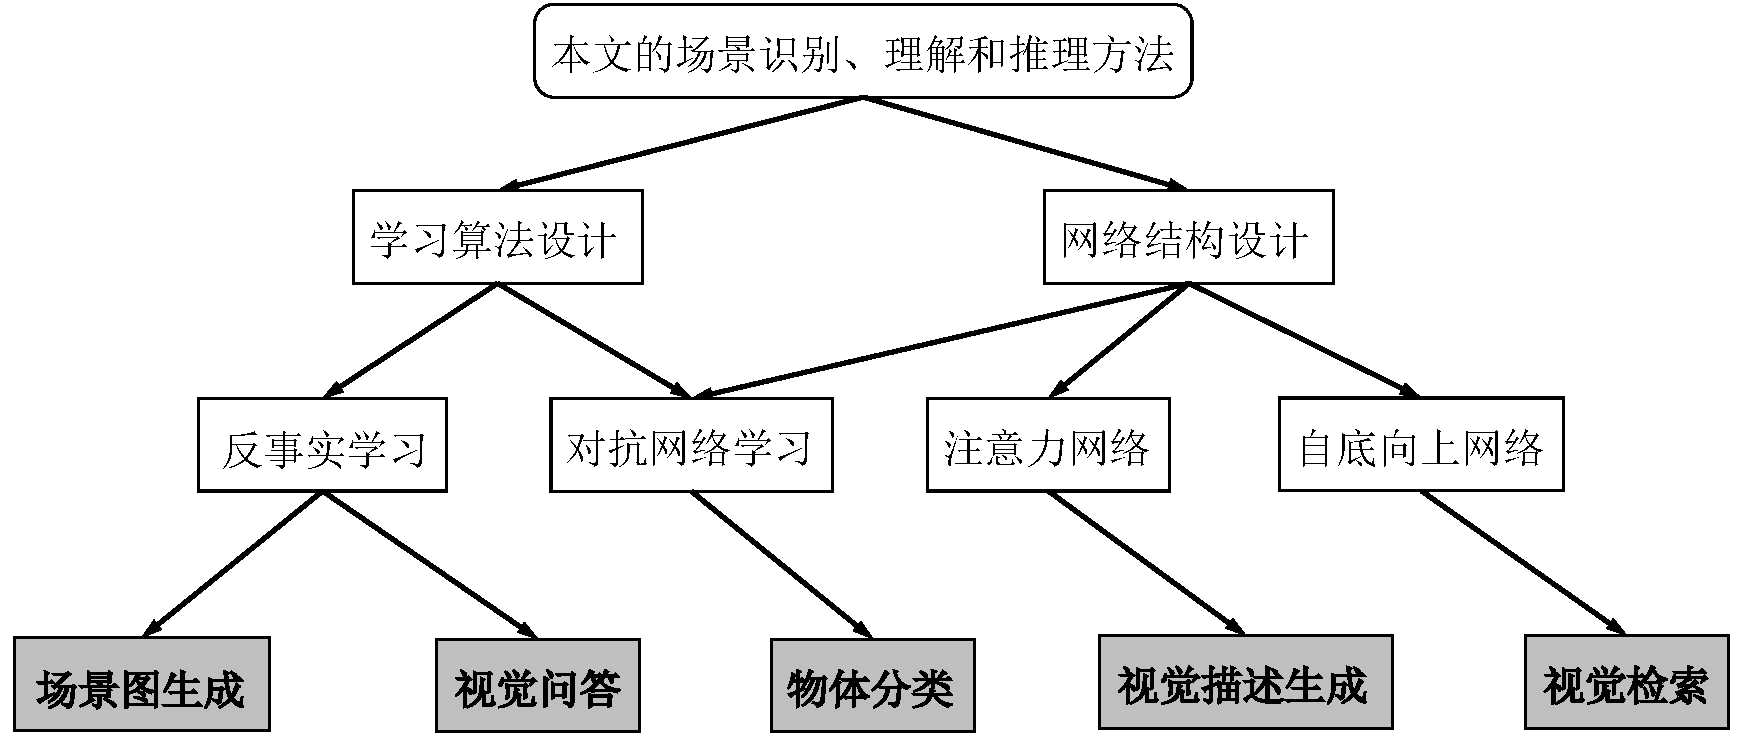
\includegraphics[width=0.95\linewidth]{chapter1/res/technique_summary.pdf}
    \centering
    \caption{复杂场景识别、检测和推理的关键技术研究方法}
    \label{ch1:fig:technique_summary}
\end{figure}


\subsection{基于反事实多智能体学习的场景图生成}
在复杂场景理解中,除了需要对单个的物体进行识别,还需要检测物体间的视觉关系。图像场景图生成任务主要研究如何充分利用场景中所有物体和物体关系之间的内在联系,提升最终所有物体和视觉关系整体的检测结果。

现有的场景图生成方法基本都是将场景内所有的物体和视觉关系分类的交叉熵之和作为模型的优化目标,并将所有的物体和视觉关系的预测认为是相互独立的。这种优化目标忽略了场景中不同物体的重要性,容易使模型陷入局部最优解。本文提出一种全新的框架,将场景图生成问题看成是一种多智能体协同决策问题,其中图像中每个物体为独立的智能体。每个智能体通过预测不同的类别(动作),提升整体的场景图生成质量。同时,本文基于反事实学习,提出一种反事实基准模型,有效地对不同物体的决策分配不同的训练梯度。本文提出的反事实多智能体学习,可以显著提升物体的类别预测,进而提升整个场景图的生成质量。


\subsection{基于多层空间和通道注意力网络的视觉描述生成}

视觉描述语句生成是一种典型的视觉场景理解任务。该任务要求模型对整个视觉场景进行充分的理解,然后生成准确的自然语言描述语句。

现有的图像描述生成模型都是基于编码-解码框架(encoding-deconding framework):即利用卷积神经网络对输入图像进行编码,然后利用递归神经网络(Recurrent Neural Network, RNN)将编码的特征向量解码成自然语句。为了提升描述语句生成的质量,空间注意力机制被广泛的使用在现有的视觉描述生成模型中。这些模型只考虑在空间维度上使用注意力机制,然而,卷积神经网络的特征图(feature map)除空间维度外,还包含通道和层级两个维度。本文,提出一种全新的多层空间和通道注意力网络,充分考虑特征图的三个维度信息,大大提升编码向量的表达能力,使得模型生成更加准确的描述语句。同时,在生成语句的过程中,帮助理解卷积神经网络中特征图的变化过程。

\subsection{基于密集型自底向上框架的视觉检索}

视觉检索任务也是一种常见的视觉场景理解任务。给定一个查询(query),模型首先需要对所有的视觉场景内容进行充分的理解,然后输出与查询内容相匹配的视觉内容。在此关键技术上,我们以视频片段的检索作为切入点,研究基于查询的视频片段检索任务。

本文首先分析了现有基于查询的视频片段检索的主流框架(自顶向下模型和稀疏型自底向上模型)的优缺点,针对目前稀疏型自底向上模型的设计缺陷,我们提出了一种全新的密集型自底向上框架。该框架包含一个密集型头网络,通过将边界预测问题分解成相关性预测和边界回归两个问题,大大降低了模型对视频动作边界定位的难度。同时,我们提出一个基于图卷积的特征金字塔层,来增强骨干网络编码的特征。该框架大大提升了自底向上模型的检索准确率。对于两种不同的查询输入(自然语句和视频片段)任务,本文提出的密集型自底向上模型都达到了目前最先进水平。

\subsection{基于反事实样本生成的视觉问答}

视觉场景理解的最终目标就是能够做到视觉推理。视觉问答是一个典型的视觉推理任务,通过对场景相关的内容进行提问,模型需要充分理解场景中的所有元素以及简单的逻辑推理关系。

本文针对于目前视觉问答模型中的普遍问题:模型受文本偏置影响较大,提出了一种全新的反事实样本生成机制。通过遮盖部分图像或者问句中的重要内容(图像区域或问句单词),同时更改标准答案,合成反事实样本。通过合并原始训练样本和新的反事实样本,迫使模型关注样本中被遮盖的重要内容,让模型在决策时关注正确的视觉区域和单词,提升模型的准确率和鲁棒性。本文提出的反事实样本生成机制可以无缝地运用到任意的视觉问答模型中,帮助提升模型回答准确率。

\section{本文组织结构}
本文通过对复杂视觉场景理解中的识别、检测和推理中的一系列典型问题,提出了多个新的优化算法和网络结构。全文共分为八章,后续章节安排如下:

\begin{asparaitem}

\item 第二章介绍了与本文相关的关键技术研究,就零样本物体分类、图像场景图生成、图像描述语句生成、视频片段检索和视觉问答等几方面的相关工作和本文的关系进行综述。

\item 第三章介绍了基于属性保持的对抗网络学习的零样本物体分类方法。本章首次提出图像分类与图像重建本质上是相互冲突的两个子任务。算法通过利用对抗学习的思想,对图像分类语义特征与图像重建语义特征进行对抗学习,让图像分类语义特征能够像图像重建语义特征保持尽量多的属性,进而提升零样本物体分类的结果。此项工作发表在国际顶级计算机视觉会议CVPR上.

\item 第四章介绍了基于反事实的多智能体学习的图像场景图生成方法。本章首次提出将场景图生成任务转化为多智能体协同决策任务,直接将整个场景图的生成质量当成优化目标,有效地对不同物体的预测类别赋予不同的梯度,显著提升物体类别的预测性能和整体场景图的生成质量。此项工作发表在国际顶级计算机视觉会议ICCV上。


\item 第五章介绍了基于多层空间和通道注意力网络的图像描述语句生成方法。本章首次提出通道注意力机制,通过对图像卷积网络的特征图在通道维度进行加权,让模型能关注到不同通道的语义信息。通过融合空间注意力机制和通道注意力机制,本章提出一种全新的多层空间和通道注意力网络,不仅极大地提升了描述语句的生成质量,也加深了人们对卷积网络特征图的理解。此项工作发表在国际顶级计算机视觉会议CVPR上。


\item 第六章介绍了基于密集型自底向上网络的视频片段检索方法。本章首次提出了一种密集型自底向上网络框架。通过提出全新的密集型头网络,解决了现有稀疏型自底向上网络框架的所有缺点。同时,本章提出一个图特征金字塔层,来增强查询和视频融合后的特征序列。通过结合密集头网络和图特征金字塔层,显著地提升了检索结果。此项工作发表在国际顶级人工智能会议AAAI上。


\item 第七章介绍了基于反事实样本生成的图像视觉问答方法。本章首次提出了一种通用的反事实训练样本生成方法,让视觉问答模型在决策时能够更加关注正确的图像区域或问句单词,提升视觉问答准确率和模型的鲁棒性。提出的样本生成方法可以无缝地运用于多种图像视觉问答模型中,持续地提升回答准确率。此项工作已经投稿至国际顶级计算机视觉大会CVPR上。


\item 第八章对全文介绍的工作进行了总结,并提出了对进一步对复杂场景理解的识别、检测和推理的研究内容以及今后的研究展望。

\end{asparaitem}


\section{本章小结}
本章对复杂视觉场景的识别、检测和推理问题进行了叙述,分别介绍了研究背景、本文的主要研究内容以及全文的组织结构。

